% ---- Don't modify from Line no. 2 to 74 ----
\documentclass[12pt]{article}

\usepackage{lineno,hyperref}
\modulolinenumbers[5]
\usepackage{graphics}
\usepackage{graphicx}
\usepackage{cite}
\usepackage{epsfig}
\usepackage{amsmath}   
\usepackage{amssymb}
\usepackage{placeins}
\usepackage[linesnumbered,ruled,vlined]{algorithm2e}
\usepackage{setspace}
\usepackage{multirow}
\usepackage[export]{adjustbox}[2011/08/13]
\usepackage{tabularx}
\usepackage{algcompatible}
\usepackage{caption}
\usepackage{epsf}
\usepackage{epstopdf}
\usepackage{subfigure} 
\usepackage{colortbl}
\usepackage{longtable}
\usepackage{enumerate}
\usepackage{tabularx, booktabs}

\usepackage[table,xcdraw]{xcolor}

\usepackage{tikz}
\usepackage{multirow}
\usepackage{enumitem}
\usepackage{soul}
\usepackage{xcolor}
\usepackage[utf8]{inputenc}
\usepackage{placeins}
\usepackage{makecell}
\newcounter{qcounter}
\usepackage{tcolorbox}
\usepackage{lscape}
\usepackage{url}
\usepackage{hyperref}
\usepackage{tablefootnote}
\usepackage{url}
\usepackage{geometry}
\usepackage{listings}
 \geometry{
 a4paper,
 total={170mm,257mm},
 left=20mm,
 top=20mm,
 }

\usepackage{hyperref}
\hypersetup{
    colorlinks=true,
    linkcolor=blue,
    filecolor=magenta,      
    urlcolor=cyan,
}

\setlength{\parindent}{4em}
\setlength{\parskip}{1em}
\renewcommand{\baselinestretch}{1.5}

\usepackage[numbers]{natbib}
\bibliographystyle{unsrtnat}

\begin{document}

% ------------ Don't modify anything up to here ---------------

% From here on-wards modify only the relevant fields, such as Title (line no. 76), "Section:", "Course Instructor:", and "Team Members:" field. (Team Members details should be in the format such as, name, reg. no., mobile no. and email id.). Further, "Title:" can be changed as per your selected topic name. 

% Follow the comments properly

% All \hl{...} line at the end of report delete or comment it.

\begin{center}
    \textbf{\Large{Final Report \\
    (\textcolor{blue}{Hotel Management System})}}
\end{center}

\noindent 
\textbf{Course Code:} CS110 
\hspace{2in} 
\textbf{Course Title:} Computer Programming \\
\textbf{Semester:} B. Tech 2$^{nd}$ Sem 
\hspace{1.6in} 
\textbf{Section:} S1 \\
\textbf{Academic Year:} 2019-20 
\hspace{1.8in} 
\textbf{Course Instructor:} B. R. Chandavarkar \\
\textbf{Team Members:} \\
\textbf{1.} Gautam Shah, ME252, 9098675432, abcd@gmail.com 
\newline
\textbf{2.} Amir Khan, CH500, 9097675432, pqrs@gmail.com

\vspace{0.25in}

\section{Abstract}

\hl{Write the abstract (what you submitted in abstarct document) of your report here}

\newpage                % Don't delete
\section{Introduction}  % Don't delete

\hl{Write the introduction (detail of abstract) to your mini-project}

\newpage                            % Don't delete
\section{Flowchart or Algorithm}    % Don't delete

\hl{Enclose the flowchart of your mini-project}

\newpage                            % Don't delete
\section{Source Code}               % Don't delete

\hl{Enclose the source code of your programs as per the below shown example.}

This section of the report presents the source for finding the factorial of input number using recursive function.

\noindent \textbf{1. fact.c}

% between \begin{lstlisting} and \end{lstlisting} include your source code of one .c file. The same you repeat to add other .c file source code

\begin{lstlisting} 
#include<stdio.h>
long int multiplyNumbers(int n);
int main() {
    int n;
    printf("Enter a positive integer: ");
    scanf("%d",&n);
    printf("Factorial of %d = %ld\n", n, multiplyNumbers(n));
    return 0;
}

long int multiplyNumbers(int n) {
    if (n>=1)
        return n*multiplyNumbers(n-1);
    else
        return 1;
}

#include<stdio.h>
long int multiplyNumbers(int n);
int main() {
    int n;
    printf("Enter a positive integer: ");
    scanf("%d",&n);
    printf("Factorial of %d = %ld\n", n, multiplyNumbers(n));
    return 0;
}

long int multiplyNumbers(int n) {
    if (n>=1)
        return n*multiplyNumbers(n-1);
    else
        return 1;
}

#include<stdio.h>
long int multiplyNumbers(int n);
int main() {
    int n;
    printf("Enter a positive integer: ");
    scanf("%d",&n);
    printf("Factorial of %d = %ld\n", n, multiplyNumbers(n));
    return 0;
}

long int multiplyNumbers(int n) {
    if (n>=1)
        return n*multiplyNumbers(n-1);
    else
        return 1;
}
\end{lstlisting}

\hl{Similarly you can add other files (.c) as shown above with proper numbering and name of the file.}

\newpage            % Don't delete
\section{Results}   % Don't delete

\hl{Enclose the snapshots of your results.}

\begin{figure}[h!]
    \centering
    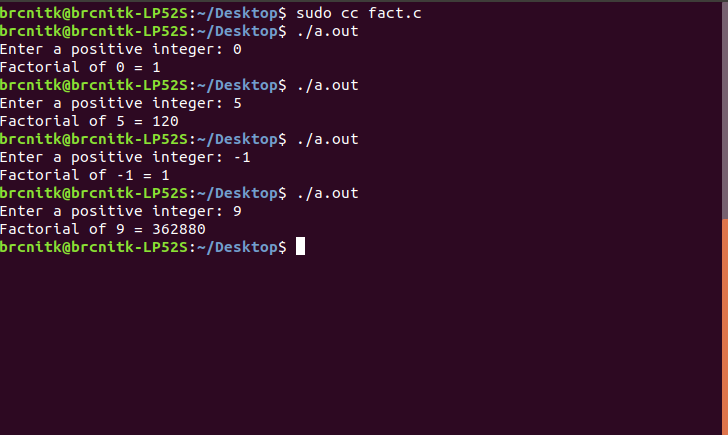
\includegraphics[width = \columnwidth]{output.png} % Here output.png is the file name of your snapshot. So, change only output.png with your file name and \caption{} to give some name. Don't touch other lines between \begin{figure} and \end{figure}
    \caption{Factorial of a input number}
\end{figure}

\newpage
\section{References:}
\begin{enumerate}
    \item http://services.lovelycoding.org/hotel-management-system/
    \item https://1000projects.org/hotel-management-system-project.html
\end{enumerate}


\begin{center}
    \textbf{**** END ****}
\end{center}

\end{document}
